\begin{center}
    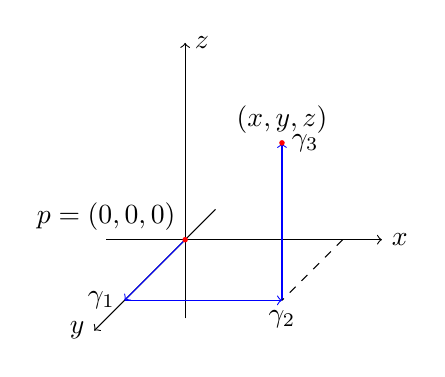
\begin{tikzpicture}
        \draw[->] (-1,0,0) -- (2.5,0,0) node[right] {$x$};
        \draw[->] (0,-1,0) -- (0,2.5,0) node[right] {$z$};
        \draw[->] (0,0,-1) -- (0,0,3) node[left] {$y$};
        %\node at (-1.2,0.5,0) {$p=(0,0,0)$};
        %\node at (2,2.5,2) {$(x,y,z)$};
        \draw[blue][->] (0,0,0) -- (0,0,2) node[black][left] {$\gamma_1$};
        \draw[blue][->] (0,0,2) -- (2,0,2) node[black][below] {$\gamma_2$};
        \draw[blue][->] (2,0,2) -- (2,2,2) node[black][right] {$\gamma_3$};
        \draw[dashed] (2,0,0) -- (2,0,2); % Linea discontinua
        \fill[red] (0,0,0) circle (1pt) node[black][above left] {$p=(0,0,0)$}; % Punto
        \fill[red] (2,2,2) circle (1pt) node[black][above] {$(x,y,z)$}; % Punto
    \end{tikzpicture}
\end{center}